\section{Design}\label{sec: Design}
In this section the design and decisions that where made to achieve the laboratory are discussed.

\subsection{Part I - RGB LED Driver}\label{subsec: Jupyter Notebook}
From project description, create the RGB LED color mixer using the ipywidgets integer or float slider. In theory, you should be able to create an infinite amount of colors with the combination of red, blue, and green LEDs. However, with digital electronics, we are limited to the width of the driving data bus or processing system to create the colors. The Project description states the following \cite{Parikh2018}\\

• Create individual methods for enabling/disabling RED, GREEN and BLUE color of the RGB LED.\\

• PWM functionality for color mixing of the RGB LED.\\

• Create 3 color mixing sliders using ipywidgets. One slider per color (R-G-B).\\

• Create toggle buttons for all four of the green LEDs using ipywidgets.\\

• Create a way to set a flashing rate of the green LEDs using ipywidgets.\\

• Create a neat and organized GUI for all of the LED functionality. \\

First make a back up of all files that are to be modified. The files saved are \_\_init\_\_.py, base.py, and rgbled.py. This is done with connecting a network drive to the Python Productivity for ZYNQ (PYNQ) platform and copy the files over to an computer. The reason to do so is that the files can not be accessed over the web browser. Listening \ref{lst: p1_2} shows the changes made in the init file. This file imports the renamed class myrgbled by startup of the kernel. Listing \ref{lst: p1_3} shows how the base file is modified so that instead of the original rgbled driver the modified driver myrbgbled is used.

\begin{lstlisting}[style=PythonStyle, language=Python, caption={Python code changed on line 45 of file \_\_init\_\_.py.},label=lst: p1_2]
from .myrgbled import MYRGBLED
\end{lstlisting}

\begin{lstlisting}[style=PythonStyle, language=Python, caption={Python code changed on line 99 of file base.py.},label=lst: p1_3]
self.rgbleds = ([None] * 4) + [pynq.lib.MYRGBLED(i)
                                     for i in range(4, 6)]
\end{lstlisting}

To save the on the computer modified driver file back on to the PYNQ platform an trick is needed due to the restricted access rights of the /lib folder. Listing \ref{lst: p1_1} shows how the terminal command that is used to copy (cp) the file from folder /PYNQ to /PYNQ/lib because the file can be copyed into folder /PYNQ.

\begin{lstlisting}[language=bash, caption={Jupiter Notebook terminal, copy a file.},label=lst: p1_1]
root@pynq:/home/xilinx# cp /home/xilinx/pynq/myrgbled.py /home/xilinx/pynq/lib/myrgbled.py
\end{lstlisting}
%\begin{wrapfigure}{r}{0.7\textwidth}
\begin{figure}[H]
	\centering
	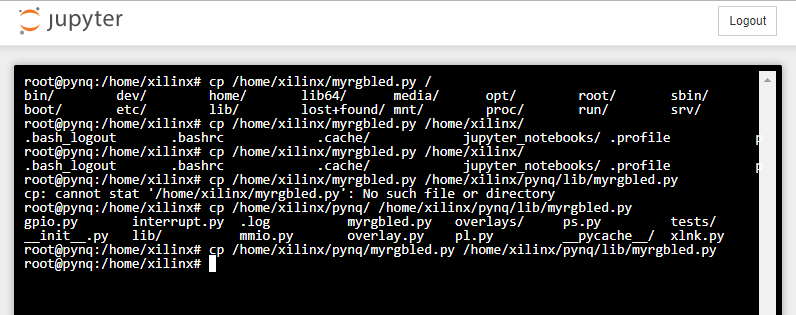
\includegraphics[width=\textwidth]{01_images/p1_terminal_cp}
	\caption{Jupiter Notebook terminal, copy a file.}
	\label{fig: part1_terminal}
\end{figure}
%\end{wrapfigure}
\fbox{\begin{minipage}{\linewidth}\large\textbf{Notice:} The original functions of the driver remind. This provides back words compatibility for previous written programs.
\end{minipage}}
\vspace{11pt}

To the driver a method for pulse width modulation (PWM) is added, shown in Listing \ref{lst: p1_pwm_rgb}. As inputs of the pwm() method a color can be defined which is either value 1, 2, or 4. Define a duty circle and a frequency to define the pulse length and period of the generated signal.
\begin{lstlisting}[style=PythonStyle, language=Python, caption={RGB LED driver PWM  method.},label=lst: p1_pwm_rgb]
def pwm(self, color, duty_cycle, frequency):    
    """PWM for single RGB LED color.
    
    Parameters
    ----------
    color : int 1, 2 or 3
    Color of RGB specified by a 3-bit RGB integer value.
    Blue  = 1
    Green = 2
    Red = 4
    duty_cycle : int between 0 and 100
    Duty cycle is an integer value between 0 and 100 %
    ____+----+____+----+____+ is a duty cyle of 50 %
    frequency : int
    Frequency defines the length of the intervall
    
    Returns
    -------
    None
    
    """        
    if color not in [1, 2, 4]:
    raise ValueError("color should be an integer value from 1, 2, and 4.")
    
    try:
        self.rgb_on(color)
        time.sleep( duty_cycle / frequency )
        self.rgb_off(color)
        time.sleep( (100-duty_cycle) / frequency)   
    except ZeroDivisionError:
        print "division by zero!"
\end{lstlisting}

The pwm() method is used in the program in an independent process so it can be run in a while loop and does not interfere with the running graphical user interface (GUI) which operates event driven, the code to build processes is shown in Listing \ref{lst: p1_pwm_rgb_overwiev}. 

\begin{lstlisting}[style=PythonStyle, language=Python, caption={RGB LED driver PWM overwiev.},label=lst: p1_pwm_rgb_overwiev]
from multiprocessing import Process
from multiprocessing.sharedctypes import Value
    
def run_pwm2():  
	# prvides PWM for RGB LED        
	try:           
		while( 1 ):
			if red_duty.value != 0:
			base.rgbleds[4].pwmd(red.value, red_duty.value, frequency.value)
			if green_duty.value != 0:
			base.rgbleds[4].pwmd(green.value, green_duty.value, frequency.value)
			if blue_duty.value != 0:
			base.rgbleds[4].pwmd(blue.value, blue_duty.value, frequency.value)
			# terminate process
			if exit.value:
			break
	except KeyboardInterrupt:
		raise

# running pwm in seperate process
try:           
	p_pwm = Process(target=run_pwm2, args=(), name='pwm2')
	p_pwm.start()
except:
	raise

# running led flash in seperate process
try:           
	p_led_flash = Process(target=run_leds, args=(), name='led_flash')
	p_led_flash.start()
except:
	raise
\end{lstlisting}


The designed GUI is shown in Figure \ref{fig: part1_gui}. The first sections controls the four green LEDs and returns the status of LED0 to LED3. The light green framed section controls the green LEDs flashing rate with the slider to the right. The four check boxes are used to enable or disable the flashing of the green led. The third section controls the RGB LED LD4 and allows color mixing with the three sliders to the right, changes the PWMs duty cycle. The slider to the left controls the frequency of the PWM. At the end is an red exit button which is used to terminate the running processes properly so that the program can be restarted without restarting or interrupting the kernel.
\begin{figure}[H]
	\centering
	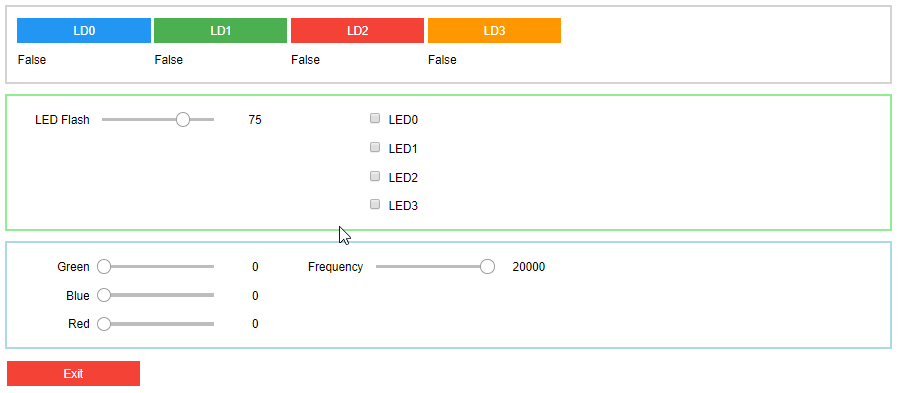
\includegraphics[width=\textwidth]{01_images/p1_gui}
	\caption{Jupiter Notebook GUI to control the green LEDs and a RGB LED.}
	\label{fig: part1_gui}
\end{figure}

It turns out that running each single color of the RGB LED is an issue if done so with three processes. The problem is that due to different duty cycles it can occur that one process invokes as example blue twice and then red only once and maybe green is not called at all. This causes the RGB color to fade in different colors then to be a stable color mixing. Therefore, the approach was changed to one process which runs the three colors sequentially. Turns out, this method works quite well.
Due to the fact that two different process where used and each process has an independent Heap global variables aren't shared anymore and the class Value had to be used to synchronize those. For a larger project certainly a queue would be more appropriate to handle values between processes. An different approach would be instead of using processes to start two threads which would have the same Heap but might come with the price of decreased performance. By using a process it is important to implement a small delay from time.sleep. 

The full code is shown in the appendix Section \ref{subsec: Python code Listings Part I}.

\subsection{Part II - LED Groove Bar}\label{subsec: Part II - LED Groove Bar}
The Groove LED Bar can be turned on in level increments from 0 to 10 where 0 is off and 10 all segments on. The brightness of the leds can be defined independently with an value from 0 to 3 where 0 is off, 1 is low, 2 is medium, and 3 is led brightness high. As graphical user interface (GUI) two integer slider are used SL1 and SL2 as shown in Figure \ref{fig: part2_output}. The source code is shown in Listing \ref{lst: Python Part 2} in Section \ref{subsec: Python code Listings Part II} of the appendix.

%\begin{wrapfigure}{r}{0.7\textwidth}
	\begin{figure}[H]
	\centering
	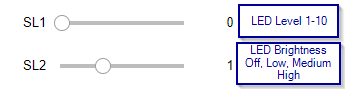
\includegraphics[width=0.6\textwidth]{01_images/p2_gui}
	\caption{Groove LED Bar program output.}
	\label{fig: part2_output}
	\end{figure}
%\end{wrapfigure}

\subsection{Part III - Music Synthesizer}\label{subsec: Part III - Music Synthesizer}

To build a music synthesizer first the overlay and necessary python functions are loaded in the first cell. 

\subsubsection{MicroBlaze Softcore for PMODA} 
Second, a magic cell is build with the magic MicroBlaze command, shown in Listing \ref{lst: p3_microblaze}. The microblaze cell works as a C wrapper for python as well as it allows to write C code and function which will be compiled, flashed, and executed on the MicroBlaze softcore.

The cell compiles, flashes, and executes C code on the MicroBlaze softcore. Each peripheral outlet, as they are PMODA, PMODB, and ARDUINO has there own MicroBlaze.

The cell uses the PMODA MicroBlaze to execute driver code which allows the programmer to invoke C functions directly in python code. This works of because of cell magic, where the MicroBlaze cell wraps the C function to make it accessible for python.

Due to the fact that there is only one MicroBlaze per outlet a notebook can only have one cell per each MicroBlaze. if there more the first code will be compiled, flashed, and executed. As the the second MicroBlaze cell with the same outlet is run the C code of that cell is compiled, flashed, and executed on the MicroBlaze. 

\begin{lstlisting}[style=PythonStyle, language=Python, caption={Magic microblaze command.},label=lst: p3_microblaze]
%%microblaze base.PMODA
\end{lstlisting}

\subsubsection{C code in MicroBlaze to Play a Melody} 
The MicroBlaze cell is used to run C code that builds the drivers for the connected peripherals to the PMODA. In this case the Groove connector is connected to the PMODA and is equipped with the Groove LED Bar on connector G1 and the Groove Buzzer is connected to G4.

The init functions for buzzer and LEDs had to be written or modified because usually the driver would be compiled and run as program on the platform. Therefore,general purpose input outputs (GPIO)s had to be initialized directly as shown in Listing \ref{lst: p3_C_init}. Interesting is that the led  bar init has an counter intuitive GPIO assignment where someone would assume that clock (clk) would be pin A but pin A is the data pin and pin B is the clock pin. 
\lstset{style=CStyle}
 \begin{lstlisting}[language=C, basicstyle=\footnotesize, caption={Magic microblaze C code for buzzer and ledbar initialization .},label=lst: p3_C_init]
 void buzzer_init(){
     pb_speaker = gpio_open(PMOD_G4_A);
     gpio_set_direction(pb_speaker, GPIO_OUT);
 }
 void ledbar_init(){  
    gpio_clk = gpio_open(PMOD_G1_B);
    gpio_data = gpio_open(PMOD_G1_A);
    gpio_set_direction(gpio_clk, GPIO_OUT);
    gpio_set_direction(gpio_data, GPIO_OUT);
 }
 \end{lstlisting}
 
 To be able to play 10 tunes the buzzer function playNote() had to be expanded with one extra tune which is the lower B and the the maximum value of the for loop had to be increased from 8 to 10 as shown in Listing \ref{lst: p3_C_playNote}. In addition, the set\_bits() function is used to turn on the appropriate value on the ledbar that corresponds to the note which is buzzed.

\begin{lstlisting}[ language=C, basicstyle=\footnotesize, caption={Magic microblaze C code for playing a note.},label=lst: p3_C_playNote]
void playNote(char note, int duration) {
	
	char names[] = { 'B', 'c',  'd',  'e',  'f',  'g',  'a',  'b', 'C',  'D'  };
	int tones[] = {  2010, 1916, 1700, 1519, 1432, 1275, 1136, 1014, 956, 836 };
	int i;
	
	// play the tone corresponding to the note name
	for (i = 0; i < 10; i++) { // haringd changed to 10
		if (names[i] == note) {
			set_bits(reverse_data(0b00000000001 << i));
			playTone(tones[i], duration);
			
		}
	}
}
\end{lstlisting}

To play a melody the function melody\_demo() is changed with an individual melody the 'A-Team' theme, shown in Listing \ref{lst: p3_C_melody_demo}. The notes and beats array are changed accordingly. To turn of the ledbar the function set\_bits(0) is used if condition which handles a pause where note is played. Further adjustments where made to the tempo variable which is set to seventy two. The length is defined by the size function of the notes array. To improve a stable use by all users it is recommended to check that the length of beats and notes are equal. Note, this is done in the python version of the program.

\begin{lstlisting}[ language=C, basicstyle=\footnotesize, caption={Magic microblaze C code for playing the A-Team theme.},label=lst: p3_C_melody_demo]
void melody_demo(void) {
	// The number of notes to play
	int length = 20;

	/*  A-Team theme */
	char notes[] = {' ','C','C','g','C','f','g','c','e','g','C','g','D','C','b','a','g','f','g', ' ',\
		'C','C','g','C','e','f','d','g','c','e','f','a','b','b','a',' ','f','c','a',\
		' ','d','f','g','C','g','f',' ','g','f','f','e','c','B','c',' ',\
		'e','e','d','e',' ','d',' ','e',' ','d',' ','d','a','g',
		'e','e','d','e',' ','d',' ','c',' ','c',' ','c','d', ' '};
	int beats[] = {  8,  3,  1,  2, 18,  2,  8, 10,  1,  1,  2,  2,  2, 18,  3,  1,  1,  3, 16,  1, \ 
		3 , 1 , 2 , 18, 2 , 2 , 2 , 2 , 16, 3 , 1 , 2 , 50, 2 , 2 , 2 , 2 , 8 , 8, \
		8 , 3 , 1 , 2 , 18, 2 , 2 , 2 , 8 , 8 , 2 , 2,  2,  2,  16, 2, \
		2 , 2 , 2 , 2 , 2 , 2 , 2 , 2 , 2 , 2 , 2 , 2,  8,  8, \
		2 , 2 , 2 , 2 , 2 , 2 , 2 , 2 , 2 , 2 , 2 , 2,  16,  1 };

	length = sizeof(notes);
	int tempo = 73;
	int i;
	
	for(i = 0; i < length; i++) {
		if(notes[i] == ' ') {
			set_bits((0b00000000000));
			delay_ms(beats[i] * tempo);
		} else {
			playNote(notes[i], beats[i] * tempo);
		}
		// Delay between notes
		delay_ms(tempo / 2);
	}
}
\end{lstlisting}

For simple use a main function named c\_music\_play() is programmed that initializes the ledbar and the buzzer GPIOs. A one second blink of five leds shows the initialization was successful. The melody function is called to play the melody. The described code is shown in Listing \ref{lst: p3_C_c_music_play}.
\begin{lstlisting}[ language=C, basicstyle=\footnotesize, caption={Magic microblaze C code for playing the A-Team theme.},label=lst: p3_C_c_music_play]
void c_music_play(){
	buzzer_init();
	ledbar_init();
	set_bits(0b1111100000);
	delay_ms(1000);
	melody_demo();
}
\end{lstlisting}

After executing the MicroBlaze cell which compiles, flashes, and executes the code onto the MicroBlaze, builds python wrappers for the C functions so they can be called in python in a cell of the Jupiter notebook, the function c\_music\_play() can be used in the next cell with pressing Shift+Return the melody sounds on the buzzer and the led lights up to the corresponding note.

\subsubsection{Python melody}
In addition to the C implementation the same function was build with python by using the basic C driver functions provided by the magic MicroBlaze cell. 

Now that python is used a dictionary seems appropriate to access notes which can be made as a list as well.

To check that the LEDs are ordered and inconsistency with the led bar a gamut is programmed that also prints out the current values in console, shown in Figure \ref{fig: p3_gamut_print}.

\begin{figure}[H]
	\centering
	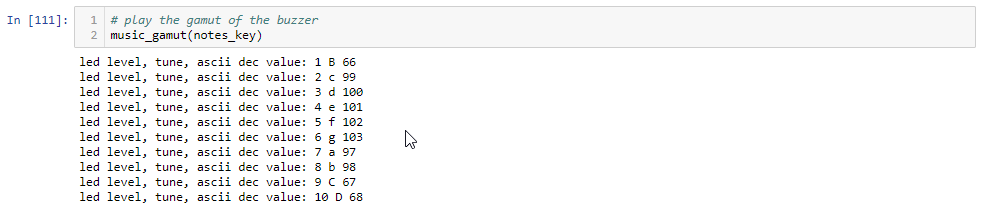
\includegraphics[width=1\textwidth]{01_images/p3_gamut_print}
	\caption{GUI for an simple music synthesizer that allows the composer to design a melody.}
	\label{fig: p3_gamut_print}
\end{figure}
\newpage
Due to the simple handling of the high programming language in terms of GUIs a cooler approximation of an music synthesizer was build, shown in Figure \ref{fig: part3_gui}. The GUi allows the user to pres any combination of notes and pause with the desired beat to build his own melody. The melody build is printed out below the GUI as the 'Play Awesome' button is pressed. This allows the user to copy paste his composition so no valuable tunes are lost. further work would be a clear button or a play awesome log book (donations welcome). 
\begin{figure}[H]
	\centering
	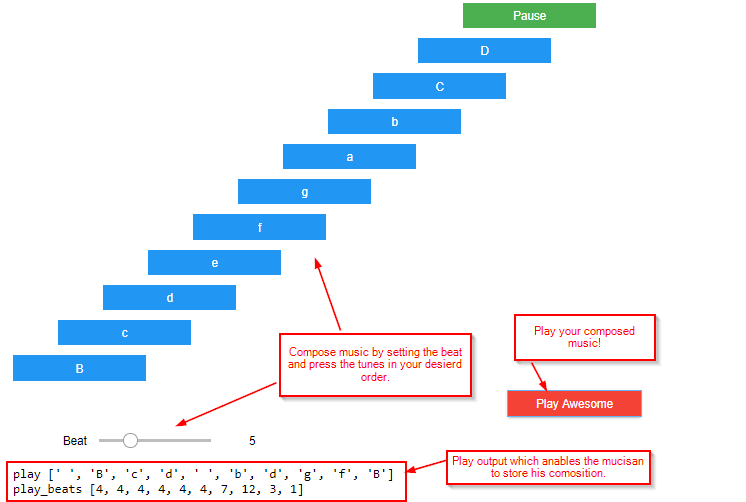
\includegraphics[width=1\textwidth]{01_images/p3_gui}
	\caption{GUI for an simple music synthesizer that allows the composer to design a melody.}
	\label{fig: part3_gui}
\end{figure}

The complete code for Part III can be found in Listing \ref{lst: MusicSynthesizer} or Section \ref{subsec: Python code Listings Part III} of the appendix.
\newpage
\subsubsection{MicroBlaze wrapper behavior}
By the programming the MicroBlaze showed interesting behavior in form that not every function was wrapped. Although, tremendous efforts where made to enlighten the mystery, no conclusive statement could be made why a function is wrapped or not. Figure \ref{fig: p3_microblaze_wrapper} shows the an example of wrapped functions and a function that would be assumed to be wrapped but is not
\begin{figure}[H]
	\centering
	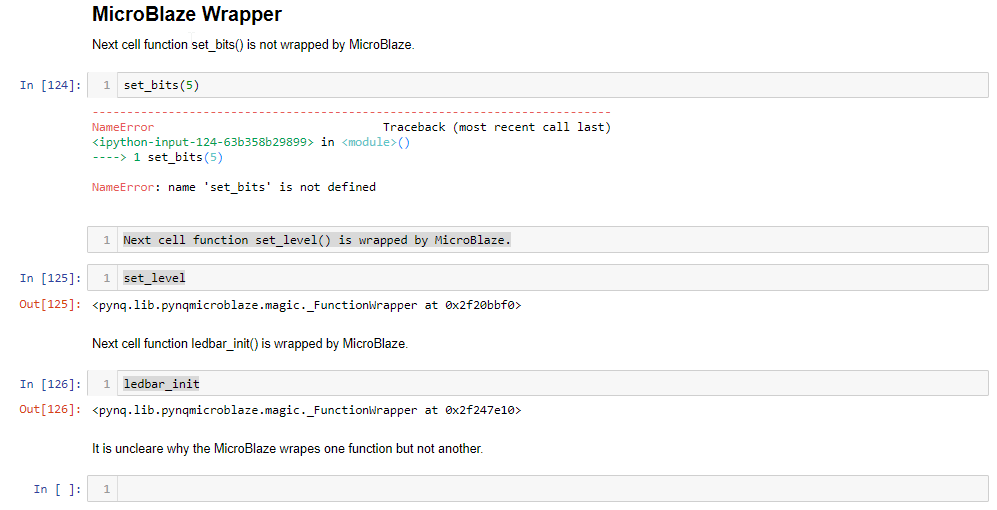
\includegraphics[width=1\textwidth]{01_images/p3_microblaze_wrapper}
	\caption{Inconsistent wrapping of C functions.}
	\label{fig: p3_microblaze_wrapper}
\end{figure}
